\documentclass[11pt,fancychapters]{article}
\usepackage[a4paper, total={6in, 8in}]{geometry}
\usepackage{cite}
\usepackage{color}
\usepackage{xcolor}
\usepackage{empheq}
\usepackage{setspace}
\usepackage{hyperref}
\usepackage{minted}
\usepackage{acro}
\usepackage{amsmath}
\usepackage{amsthm}
\usepackage{amssymb}
\usepackage{multirow}
\usepackage{graphicx}
\usepackage{geometry}
\usepackage{subcaption}
\usepackage{cancel}
\usepackage[utf8]{inputenc}
\usepackage[english]{babel}
\usepackage{tcolorbox}
\usepackage{hyperref}
\usepackage{cleveref}
\usepackage{parskip}
\usepackage{algorithm} 
\usepackage{algpseudocode} 
\usepackage{pgfplots}
 \geometry{
 a4paper,
 total={170mm,257mm},
 left=20mm,
 top=20mm,
 }
\pgfplotsset{width=8cm,compat=1.9}
\newcommand{\dbar}{{d\mkern-7mu\mathchar'26\mkern-2mu}}
\newcommand{\boxedeq}[2]{\begin{empheq}[box={\fboxsep=6pt\fbox}]{align}\label{#1}#2\end{empheq}}
\def\*#1{\mathbf{#1}}
\def\ab{ab}
\usepackage{tikz}
\usetikzlibrary{calc,trees,positioning,arrows,chains,shapes.geometric,%
    decorations.pathreplacing,decorations.pathmorphing,shapes,%
    matrix,shapes.symbols}
\geometry{top=1.3in,bottom=1.3in}

\begin{document}
\centerline{\huge{2D Project --- 50.004 Introduction to Algorithms}}

\begin{table}[ht]
\centering
\footnotesize
 \begin{tabular}{c c c c c c} 
V S Ragul Balaji&James Raphael Tiovalen&Anirudh Shrinivason&Jia Shuyi&Gerald Hoo&Shoham Chakraborty
 \end{tabular}
\end{table}

\section{Part A --- Deterministic Graph-Based Algorithm}
\subsection{Overview of Algorithm}

A solver for a 2-SAT problem can follow many methods. For a 2-SAT problem to be SATISFIABLE in Conjunctive Normal Form (CNF), every clause must be \texttt{true}. Since there are only 2 literals in each clause in a 2-SAT problem, within a single clause, we notice that we can form two implications, thus converting it into an Implicative Normal Form (INF). This sets one of the literals within the clause to be \texttt{false} and for the entire clause to be \texttt{true}, we need the other literal to be \texttt{true}. In other words, we are forbidding the four possible joint assignments of a pair of literals. This defines certain constraints between the variables, which can be propagated throughout the whole implication graph. Each pair of constraints can be considered to be an edge between the variables in an implication graph for the boolean satisfiability problem.\newline

To create the implication graph, we first implement a directed graph using an adjacency list. In the \texttt{Graph} class defined in the \texttt{dfs/kosaraju.py} file, we create the adjacency list by defining the graph's vertices, as well as a function to add edges. Since each variable produces two literals (the variable itself and its negation), we create $2n$ vertices, where $n$ is the number of variables. These vertices are added as the keys of the dictionary $G$ defined in the \texttt{Graph} class. The values for each key would be a list containing consecutive outgoing edges from the vertex defined in the key. This keeps the connection between each individual vertex to the other vertices.

\vspace{4mm}

\begin{figure}[h]\label{fig}
\centering
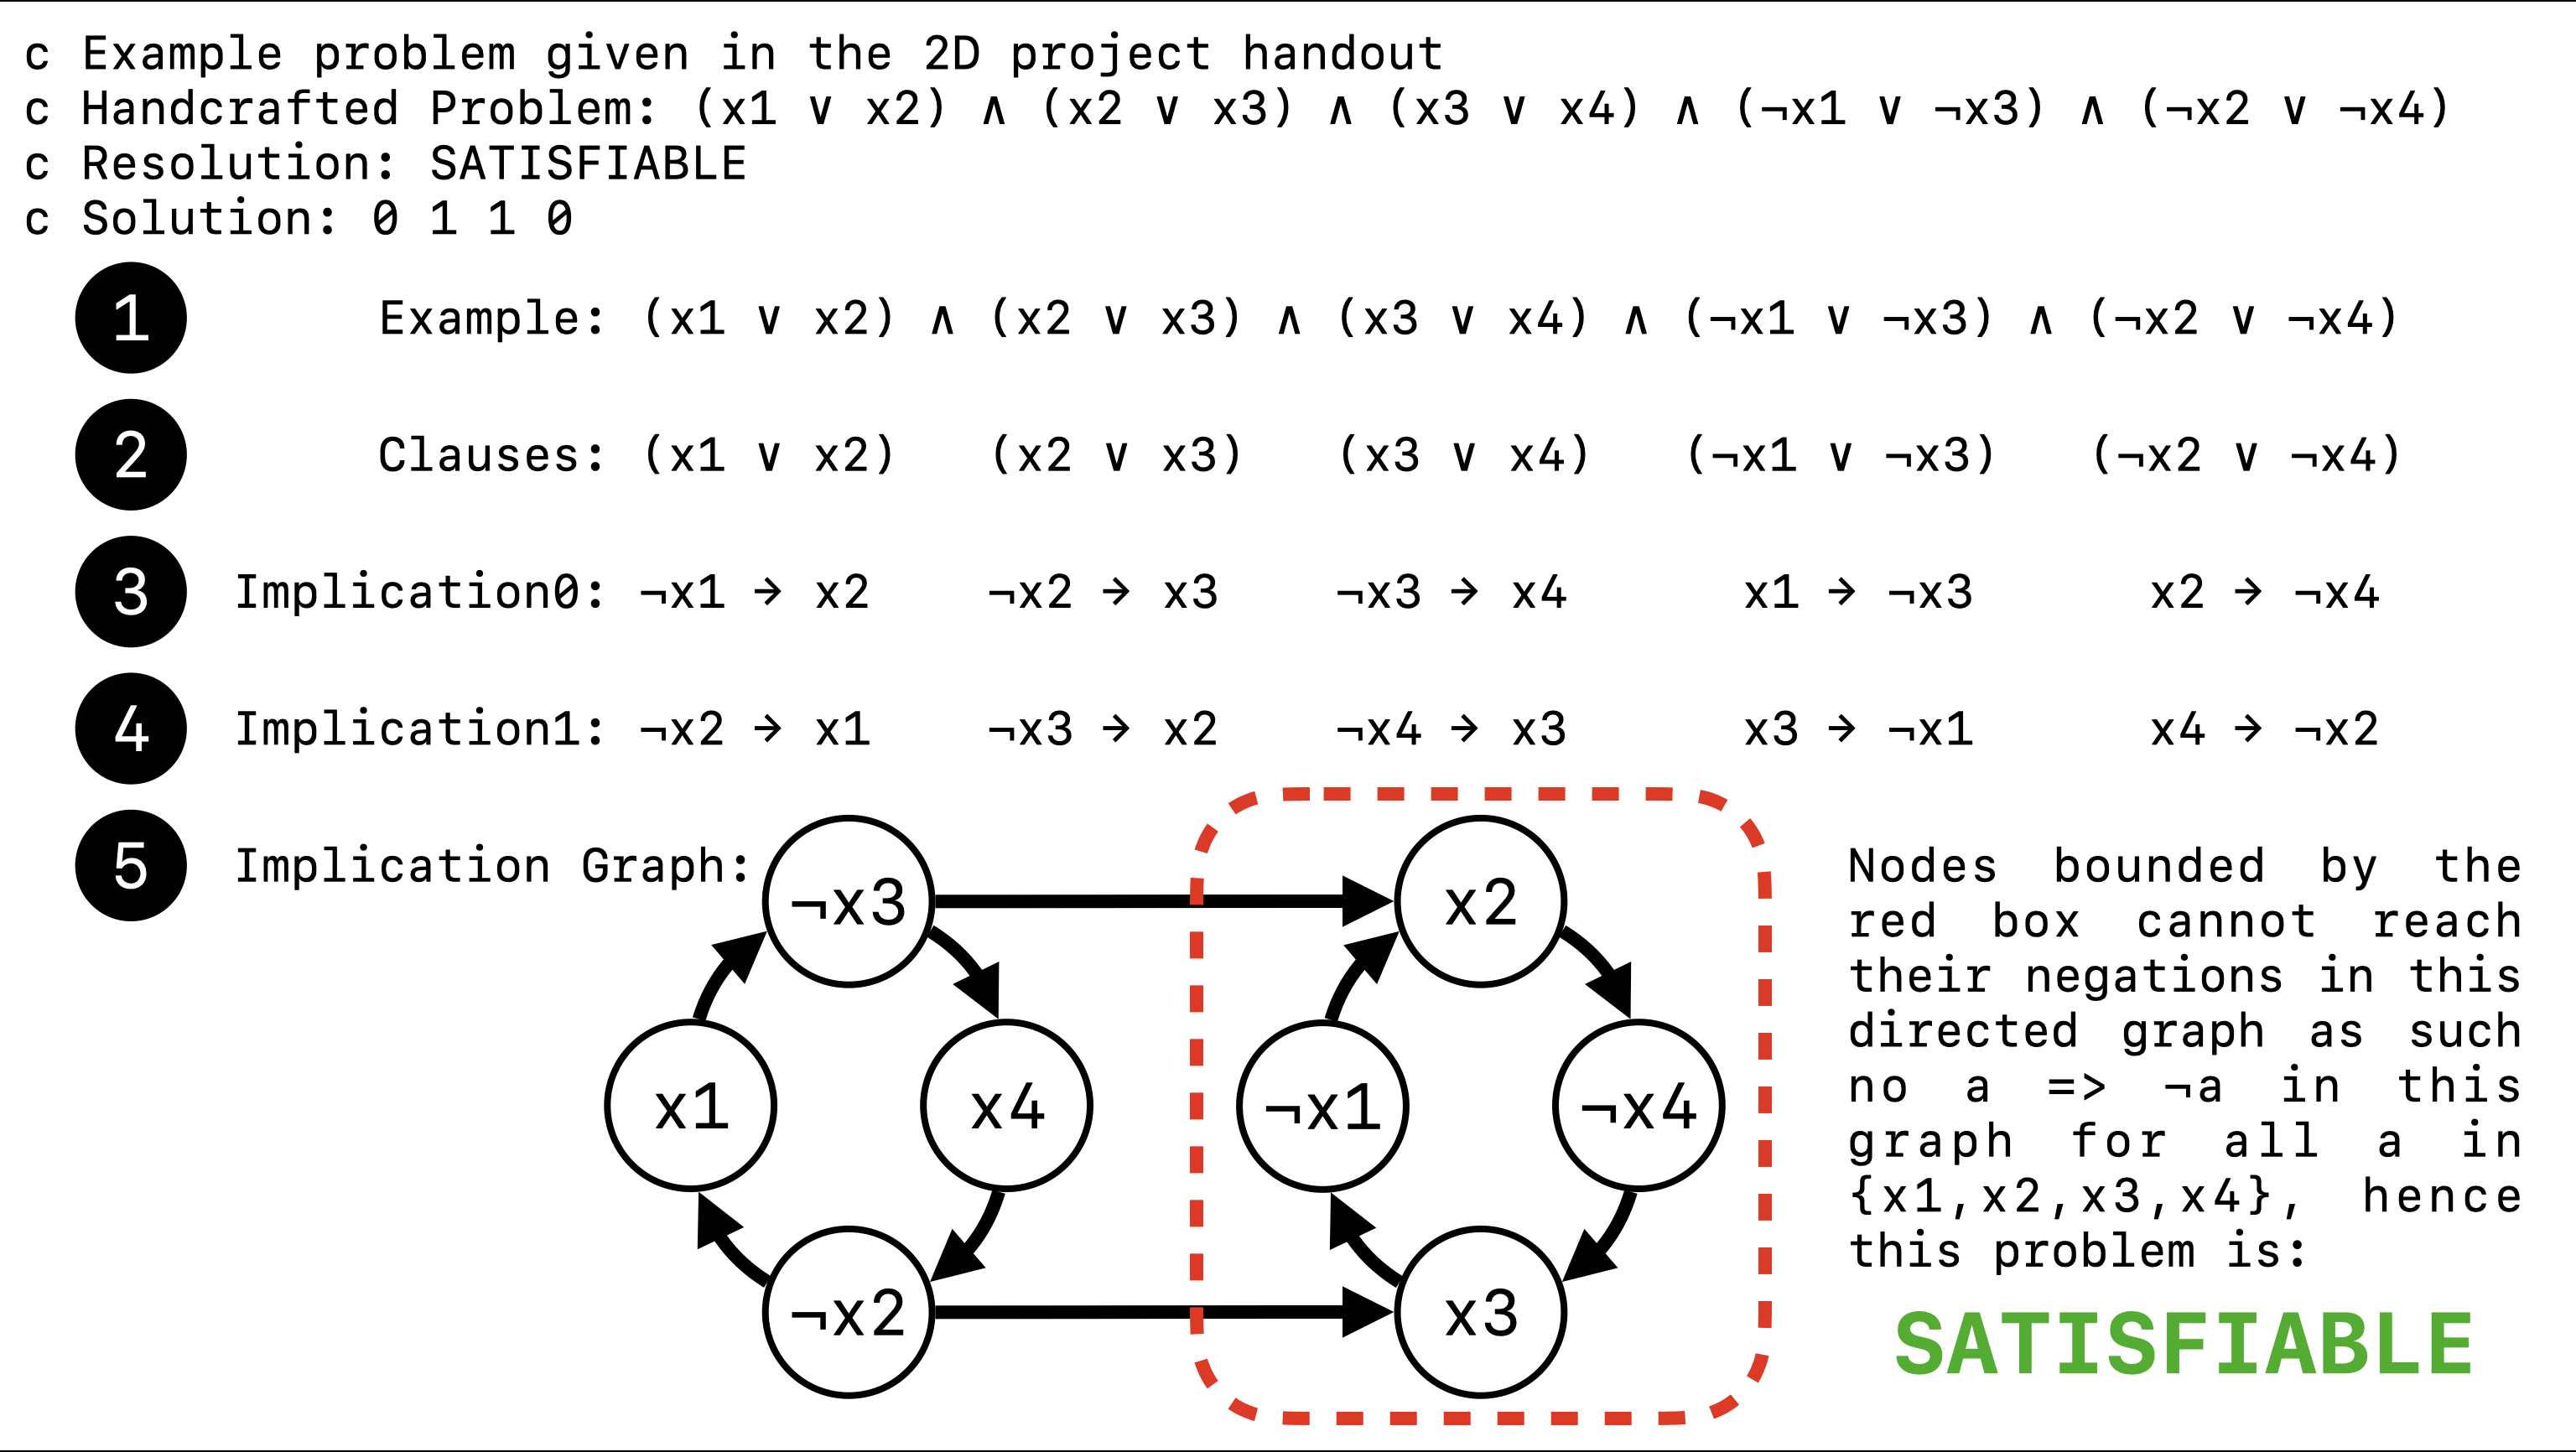
\includegraphics[width=.9\textwidth]{diagrams/example_cnf_solved.png}
\caption{Guided example of solving 2SAT by hand in polynomial time}
\label{fig:example_problem}
\end{figure}

\vspace{4mm}

In Figure~\ref{fig:example_problem}, we demonstrate this process using an example. This example is also defined in the \texttt{cnf/example.cnf} file. Steps 3 and 4 in Figure~\ref{fig:example_problem} are defined in lines 110-111 in the \texttt{kosaraju.py} file. Using the implication graph, we find the Strongly-Connected Components (SCCs) of the graph and group vertices that are along the same path using Kosaraju's Algorithm. We first create a stack and a depth-first search (DFS) is implemented to traverse through the graph. Adjacent vertices are pushed to the stack. The same procedure is executed on the inverse of the graph, where the direction of all of the edges is reversed. After that, while the stack is not empty, we pop each vertex from the stack. Using this algorithm, we can find all the SCCs of the graph.\newline

Next, we can check for contradiction in each of the SCC. If a variable and its corresponding negation is in the same SCC, the whole 2-SAT formula is deemed to be UNSATISFIABLE, as it is impossible to assign two literals to the same variable. This is because within a single SCC, you can traverse from any vertex to any other vertex. Otherwise, the formula is deemed as SATISFIABLE.\newline

If the formula is SATISFIABLE, we can output a possible solution for the formula. We can do this by grouping the SCCs together and connect them using a directed acyclic graph. Using the graph in Figure~\ref{fig:example_problem} as an example, going in topological order, assign $0$ to the first group of SCC (which is the left SCC in this specific case) and assign $1$ to the second group of SCC (the one highlighted by the red rectangle). We would then get the corresponding output of the variables by equating the literals in any SCC to the assigned value.

\subsection{Time Complexity Analysis}

In general, we know that 2-SAT is in P and is tractable due to the mechanism of forcing the other literal to be \texttt{true} in a single clause by assigning a literal within that same clause as \texttt{true}. When we pick an assignment, 3 cases could happen:

\begin{enumerate}
    \item We reach a contradiction. In this case, it means that there can only be a satisfying assignment if we use the other truth value for that specific variable. Thus, we can simplify the formula using this new assigned value for that variable and repeat the process.
    \item The ``forcing" of the value assignment for a specific variable does not affect other variables and clauses. In this case, adopt these truth values, eliminate the clauses that they satisfy and continue the process.
    \item We find a satisfying assignment.
\end{enumerate}

In Cases 1 and 2, we have spent at most $O(n^2)$ time and have reduced the length of the formula by $\geq 1$. Thus, in total, we have spent at most $O(n^3)$ time.\newline

In fact, our specific implementation method of using a DFS traversal on an implication graph using Kosaraju's Algorithm would take even less time:

\begin{enumerate}
    \item To create the implication graph, we set up the vertices and edges in $O(V + E)$ time, where $V$ is the number of vertices and $E$ is the number of edges in the graph.
    \item We implement DFS to traverse through the implication graph using Kosaraju's Algorithm in $O(V + E)$ time.
    \item We set up the inverse/transpose implication graph in $O(V + E)$ time.
    \item We implement the DFS again through the inverse implication graph in $O(V + E)$ time.
\end{enumerate}

Thus, this reduction of the 2-SAT problem to finding SCCs implemented in our deterministic algorithm would cause the algorithm to take only linear time.\newline

Meanwhile, $k$-SAT problems for $k \geq 3$ would be NP-complete (as shown by the Cook-Levin Theorem) and thus, the time taken would have non-polynomial asymptotics. This is because the size of the CNF formula is exponential in the size of the original boolean formula for $k \geq 3$.\newline

A possible improvement that could be made would be to implement Tarjan's Algorithm to conduct the search for the Strongly-Connected Components. While both Kosaraju's Algorithm and Tarjan's Algorithm would take $O(V+E)$ time, Tarjan's Algorithm has a lower constant factor to the runtime since it would need to go through the whole graph and execute DFS only once (instead of two times for Kosaraju's Algorithm, once for the normal graph and another instance of the DFS traversal for the inverse graph).

\newpage

\section{Part B --- Randomised Algorithm}
\subsection{Overview of Algorithm}
\begin{algorithm}[H]
	\caption*{\textbf{function} RANDOM\_WALK($\mathbb{F}, L$)}
	// $\mathbb{F}: \textit{a list of clauses}$\\
	// $L: \textit{a list of all variables used in } \mathbb{F}$
	\begin{algorithmic}[1]
	\State Store all variables as keys in a dictionary $\mathbb{D}$ with initial values \textbf{false}
	\For {$i \gets 1 \text{ to } 100\times(L.\textit{length})^2$}
	    \State Using $\mathbb{D}$, assign boolean values to $\mathbb{F}$
	    \State $\mathbb{C}\gets $ all invalid clauses in $\mathbb{F}$
	    \If {$\mathbb{C}.length \ne 0$}
	        \State $V\gets$ a random variable from a random clause in $\mathbb{C}$
	        \State $V\gets \neg V$
	        \State Update $\mathbb{D}$ with $V$
	   \Else
	        \State \textbf{return} SATISFIABLE
	   \EndIf
	\EndFor
	\State \textbf{return} UNSATISFIABLE
	\end{algorithmic} 
\end{algorithm}

First, we arbitrarily assign Boolean value \texttt{false} to all $n$ variables. In each of the $100n^2$ steps, we randomly choose a variable from a randomly selected invalid clause (that is, the clause evaluates to \texttt{false}) and negate its assignment. We then check if the resultant formula is satisfied or not. If no solution is found after $100n^2$ steps, we return UNSATISFIABLE. If at any point during the $100n^2$ steps the formula is satisfied, we return SATISFIABLE.
\subsection{Time Complexity Analysis}
Let $X_i$ be the number of correct assignments at step $i$. Assuming worst-case initialization, all variables are assigned incorrectly, we have $X_0 = 0$. This forces $X_1 = 1$, since flipping any variable would give us a correct assignment.\newline

For $1\le i \le n-1$, the probability for $X_i$ transiting to $X_{i+1}$ is at least $\frac{1}{2}$ while that to $X_{i-1}$ is at most $\frac{1}{2}$. This can be easily seen from the table below:

\begin{table}[H]
\centering
\begin{tabular}{|l|l|l|l|}
\hline
\multicolumn{2}{|l|}{Wrong Clause $A+B$}            & $A$           & $B$          \\ \hline
\multicolumn{2}{|l|}{Actual Value}                  & T           & T          \\ \hline
\multicolumn{2}{|l|}{Both Wrong Assignment}         & F           & F          \\ \hline
\multicolumn{2}{|l|}{One Wrong Assignment}          & F           & T          \\ \hline
\multirow{2}{*}{$P(X_i \text{ to } X_{i+1})$} & Both Wrong & \multicolumn{2}{l|}{1}   \\ \cline{2-4} 
                                       & One Wrong  & \multicolumn{2}{l|}{0.5} \\ \hline
\multirow{2}{*}{$P(X_i \text{ to } X_{i-1})$} & Both Wrong & \multicolumn{2}{l|}{0}   \\ \cline{2-4} 
                                       & One Wrong  & \multicolumn{2}{l|}{0.5} \\ \hline
\end{tabular}
\end{table}
Let us suppose the worst case – that the probability $X_i$ goes up is $\frac{1}{2}$, and down is $\frac{1}{2}$. This process is similar to a random walk.\newline

Let $h_i$ be the expected number of steps to reach $n$ on our random walk when we start at step $i$. We have
\begin{equation}\label{eqn2.1}
    h_i = \frac{h_{i-1}}{2} + \frac{h_{i+1}}{2} + 1 \quad \Rightarrow \quad h_i - h_{i+1} = h_{i-1} -h_i + 2.
\end{equation}
Using the base case $h_0 = h_1 + 1$, the next 2 steps are
\begin{align}
    h_1 - h_2 &= h_0 - h_1 + 2 = h_1 + 1 - h_1 + 2 = 3,\label{h1h2} \\
    h_2 - h_3 &= h_1 - h_2 + 2 = 3 +2 = 5,\label{h2h3}
\end{align}
where Eqn.~(\ref{h1h2}) is substituted into Eqn.~(\ref{h2h3}). By careful observation, we formulate the following expression:
\begin{equation}\label{mi}
    h_i - h_{i+1} = 2i+1.
\end{equation}
As shown above, this expression holds for $i=1$. Assume the expression is \texttt{true} for $h_k - h_{k+1} = 2k+1$ for some positive integer $k$, we want to prove that the expression holds for $i = k + 1$.
\begin{align*}
    h_{k+1} - h_{k+2} &= h_k - h_{k+1} + 2 \qquad \text{By Eqn.~(\ref{eqn2.1})}\\
    &= 2k+1+2\\
    &= 2(k+1) + 1.
\end{align*}
Thus, by mathematical induction, Eqn.~(\ref{mi}) is true for all $k \in \mathbb{Z}^+$. Using Eqn.~(\ref{mi}), we sum all the steps from $i = 0$ to $i = n$:
\begin{align*}
    h_0 &= h_n + \sum^{n-1}_{i=0}\left(h_i - h_{i+1}\right)\\
    &= \sum^{n-1}_{i=0}(2i+1)\\
    &= n+2\left(\frac{n^2-n}{2}\right)\\
    &= n^2,
\end{align*}
where $h_n = 0$.\newline

Therefore, the average time complexity of the randomised algorithm is $O(n^2)$. In other words, we will find a solution in $n^2$ steps \textbf{on average}. If we decide to run the algorithm for $2n^2$ steps, the probability of not finding a solution is at most $\frac{1}{2}$. Thus, if we run the algorithm for $100n^2$ steps (as it is in the pseudo-code), the probability of not finding a solution is $\left(\frac{1}{2}\right)^{50} = 2^{-50}$.


\newpage
\section{Performance Comparison}

\begin{figure}[h]
\centering
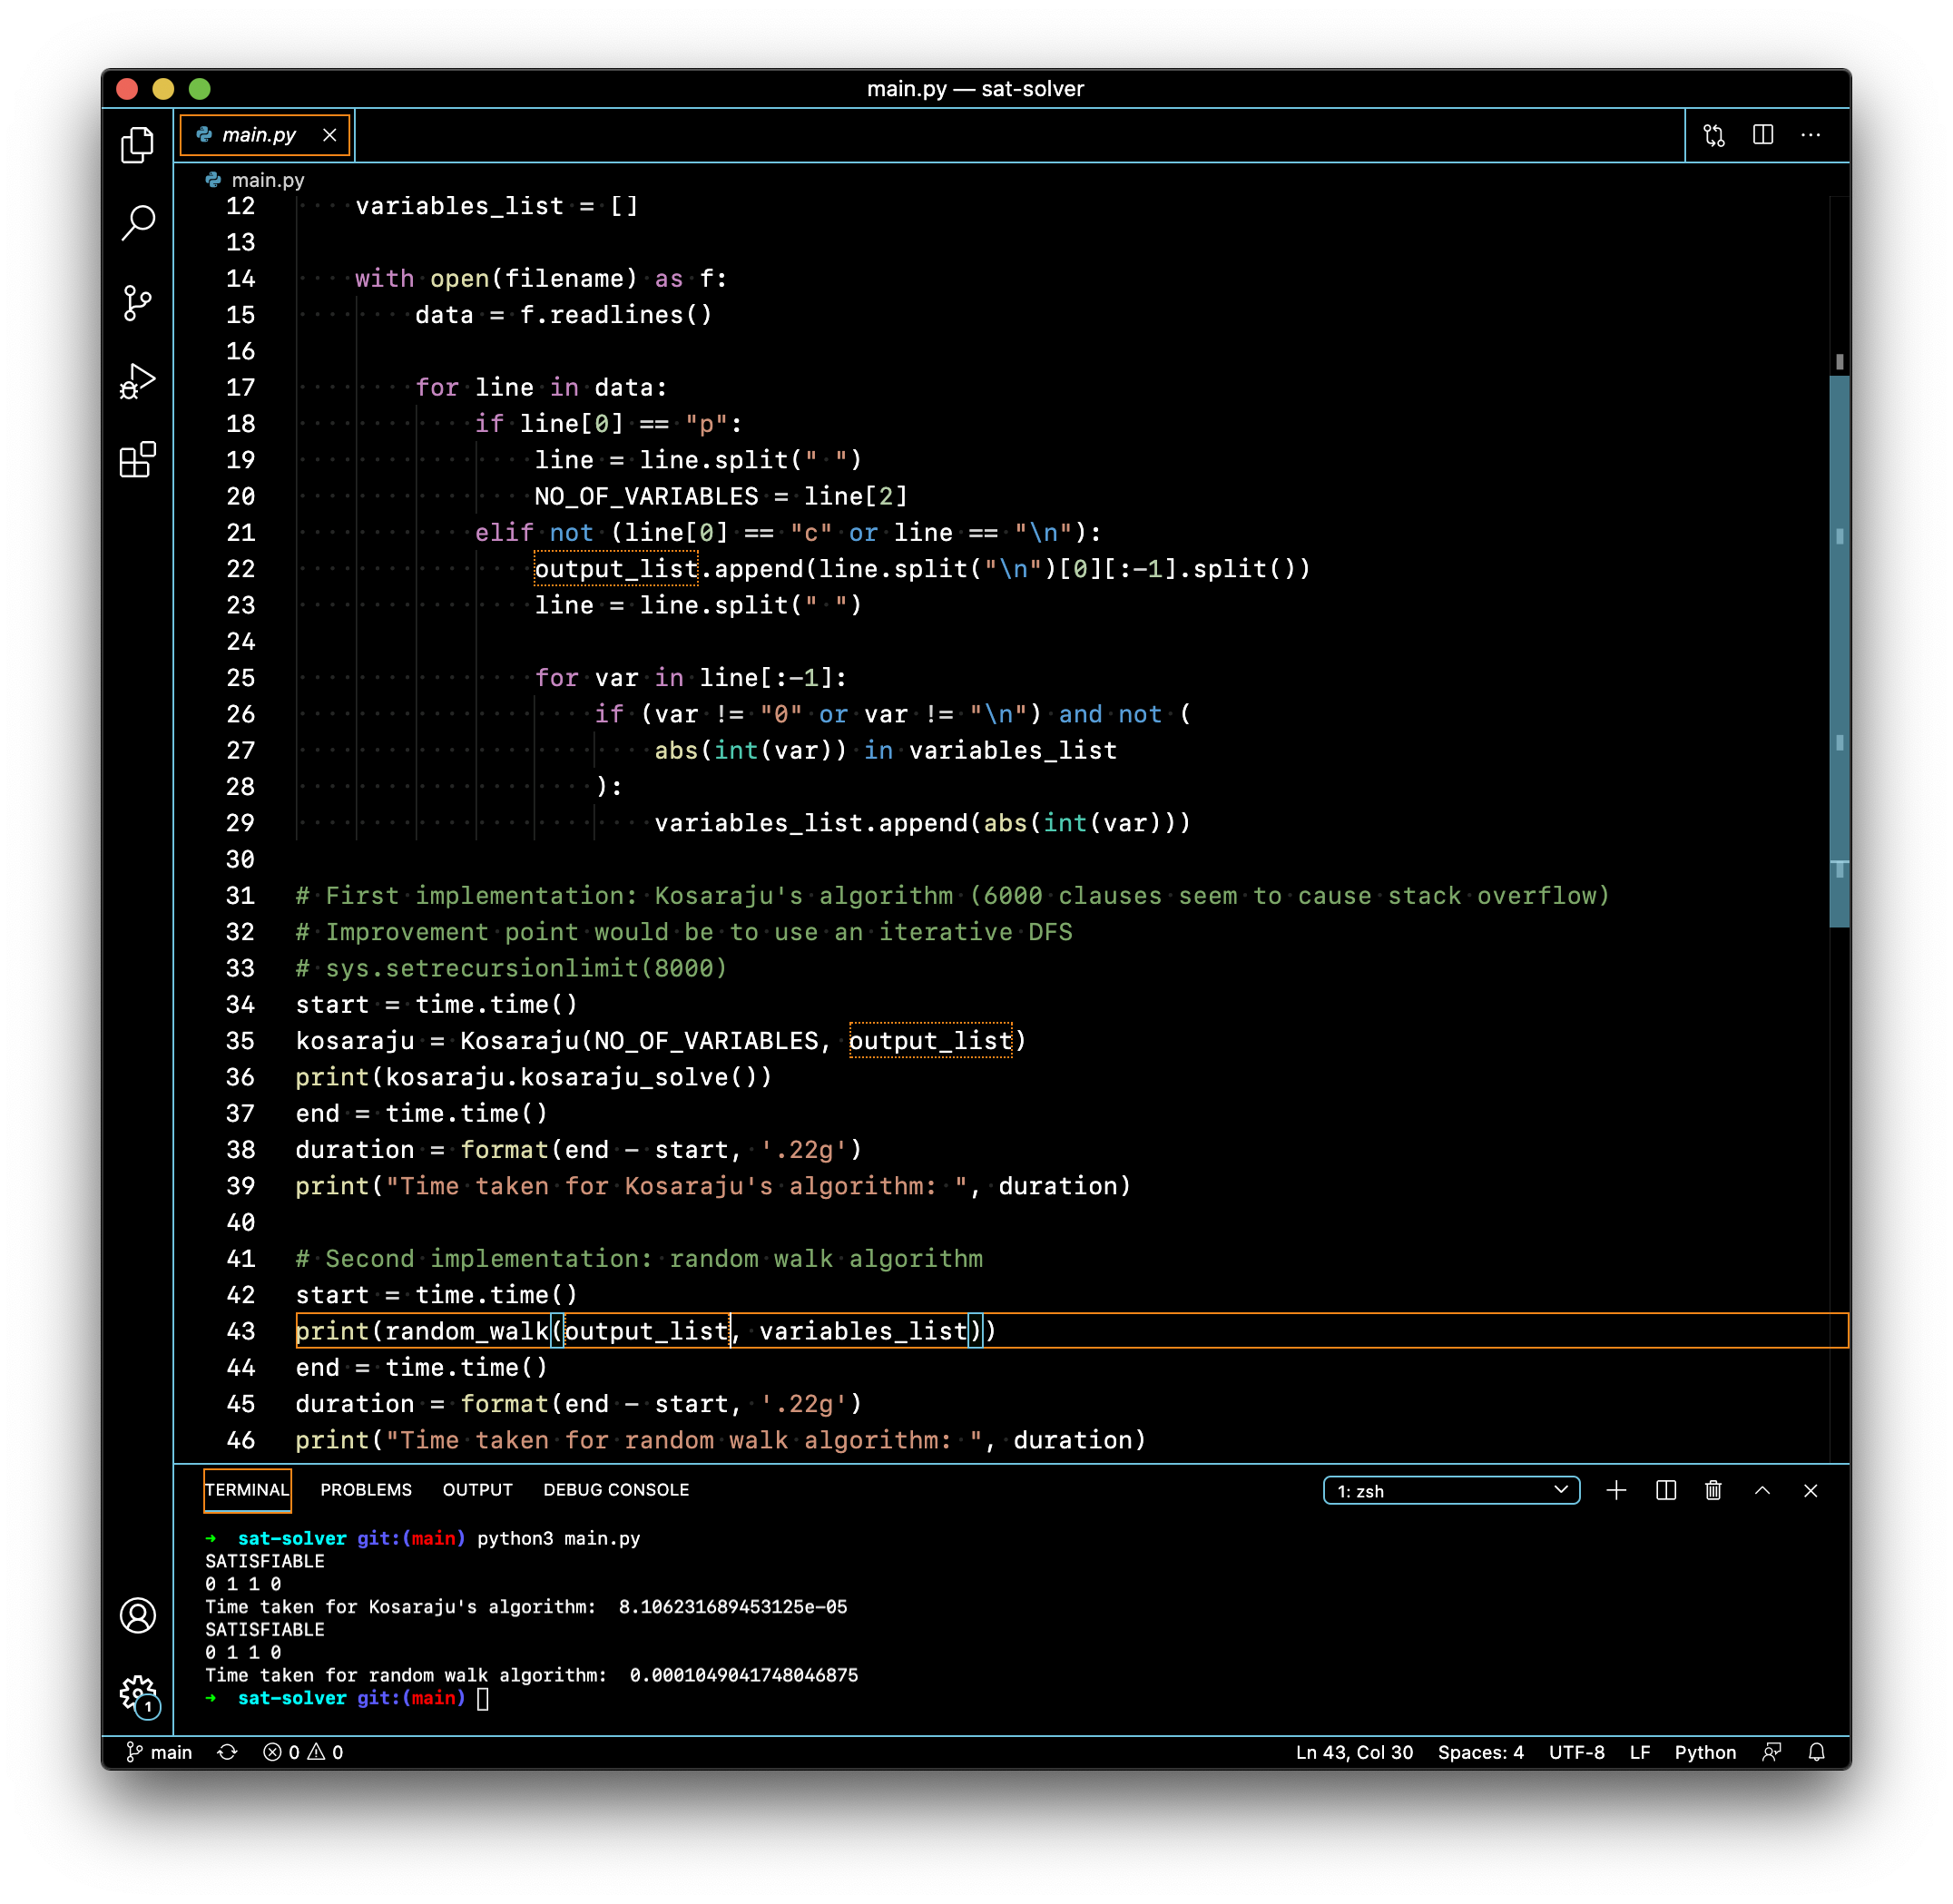
\includegraphics[width=.95\textwidth]{diagrams/test0.png}
\caption{Benchmarking script used to compare the speed of the two implementation in Part A and Part B. Kosaraju's Algorithm runs faster than the randomised algorithm as predicted by the algorithmic analysis. }
\end{figure}

\vspace{4mm}

Even though the probability of not finding a solution is very small ($2^{-50}$ for $100n^2$ steps), the randomised algorithm is not a practical substitute for the deterministic one since it takes longer time than the deterministic algorithm. There is also some chance that a solution is not found and hence an incorrect conclusion/statement of the problem's satisfiability could be made. The randomised algorithm is also dependent on the size of the variables.\newline

However, we should not dismiss the usefulness of the idea of randomised local search entirely. We should be aware that the strategy of using randomised local search is useful to improve over naive brute-force search for NP-complete $k$-SAT problems, such as the $3$-SAT problem. In fact, for a 3-SAT problem, the naive brute-force method would take $O(2^n)$ time, while a version of the randomised local search with a clever twist (such as Sch\"{o}ning's stochastic local search algorithm) would take $O\left(\frac{4}{3}^n\right)$ time, which is significantly better than $O(2^n)$.

\end{document}